We evaluate \checkcell{} across two dimensions: its execution time,
and its effectiveness at finding actual errors.

Our experimental platform is a 13'' MacBook Air equipped 4GB of RAM
and an Intel Core i5-2557M processor running at 1.70GHz. The operating
system is Windows 7 Professional (SP1), which executes non-virtualized
(via Bootcamp). \checkcell{} was compiled using Microsoft Visual C\#
2010, and runs as an add-in in Microsoft Excel 2010.

\subsection{Execution Time}
\label{sec:execution_time}

To measure the runtime of \checkcell{}, we run it on a random subset
of 30 spreadsheets drawn from those spreadsheets in the EUSES
spreadsheet corpus~\cite{Fisher:2005:ESC:1082983.1083242} that contain
formulas.

Table~\ref{tab:spreadsheet_characteristics} includes
characteristics of these spreadsheets, ordered by the number of
formulas each contains. The raw number of cells is the number of cells
that participate in any computation; the weighted number of cells is
the number of cells weighted by the number of times each cell is used
in a computation. For example, a cell that is involved in two
computations is counted twice.

Figure~\ref{fig:datadebug_runtime} reports the performance of data
debugging across our spreadsheet suite, ordered by the weighted number
of cells.

As our analysis in Section~\ref{sec:asymptotic_analysis} predicts, the
cost of \checkcell{} is dominated by impact analysis, which is in turn
dependent on the weighted number of cells.

For almost all of the spreadsheets, \checkcell{} takes less than 15
seconds to complete its analysis. In only FIXME cases, \checkcell{}
takes more than a minute; the longest runtime we observe is for the
spreadsheet FIXME, which required FIXME minutes to run.

This outlier FIXME....

\begin{table}[t!]
  \centering
    \begin{tabular}{l|rrr}
      \bf{Spreadsheet} & \textsf{\bf{Formulas}}  & {\bf{Cells}}       & {\bf{Cells}} \\
                       &                         & {\small{\it{raw}}} & {\small{\it{weighted}}} \\
    \hline
\small{3660 schedule S2003} & \small{31} & \small{1} & \small{0} \\ 
\small{ReqComp} & \small{54} & \small{162} & \small{0} \\ 
\small{Inventory\_Control} & \small{33} & \small{21} & \small{0} \\ 
\small{RMRanker95} & \small{79} & \small{54} & \small{11} \\ 
\small{Logistikkostnader} & \small{73} & \small{29} & \small{26} \\ 
\small{HMWK112403} & \small{36} & \small{41} & \small{27} \\ 
\small{30day} & \small{125} & \small{92} & \small{30} \\ 
\small{2002fairreport} & \small{3} & \small{39} & \small{39} \\ 
\small{9620040303160820} & \small{42} & \small{81} & \small{81} \\ 
\small{Inventory errors} & \small{100} & \small{129} & \small{90} \\ 
\small{grades} & \small{227} & \small{661} & \small{96} \\ 
\small{expenses\_ans} & \small{57} & \small{60} & \small{120} \\ 
\small{grades2002} & \small{61} & \small{143} & \small{123} \\ 
\small{csDept-PayrollTimecardEntry} & \small{68} & \small{204} & \small{124} \\ 
\small{Example\_3} & \small{71} & \small{130} & \small{127} \\ 
\small{lmc\_financial} & \small{72} & \small{148} & \small{142} \\ 
\small{104r} & \small{22} & \small{146} & \small{144} \\ 
\small{TRAIL INVENTORY N\#A850A} & \small{2} & \small{156} & \small{156} \\ 
\small{Grades-6\_excerpt} & \small{106} & \small{168} & \small{168} \\ 
\small{intresults} & \small{1066} & \small{3158} & \small{239} \\ 
\small{OakProducts} & \small{69} & \small{271} & \small{242} \\ 
\small{am\_skandia\_fin\_supple\#A80EE} & \small{56} & \small{272} & \small{268} \\ 
\small{E04\_AppE\_Census\_Database\_50} & \small{42} & \small{300} & \small{300} \\ 
\small{pfi-anxa} & \small{5} & \small{310} & \small{310} \\ 
\small{q exhibit54-OEA} & \small{797} & \small{1160} & \small{365} \\ 
\small{econ424-fall2003-publ\#A8A23} & \small{93} & \small{517} & \small{384} \\ 
\small{Grades\_EEE481\&581} & \small{177} & \small{757} & \small{756} \\ 
\small{gpa\_calculator} & \small{80} & \small{80} & \small{819} \\ 
\small{s446gradessp04} & \small{335} & \small{1369} & \small{1247} \\ 
\small{NEW} & \small{2626} & \small{2574} & \small{2403} \\ 
    \hline
    \end{tabular}%
  \caption{The benchmark suite of spreadsheets (a random sample from the EUSES repository~\cite{Fisher:2005:ESC:1082983.1083242}), ordered by weighted number of cells. The raw number of cells indicates the number of cells that are used in any formula; the weighted number of cells weighs each cell by the number of formulas that depend on it.\label{tab:spreadsheet_characteristics}}
\end{table}

% Info about the benchmarks.

% \subsection{Benchmarks}

%\subsection{Case Studies}

% \paragraph{9-Grades}

\subsection{User Study}
\label{sec:user_study}

We perform a user study to evaluate \checkcell{}'s efficacy at finding
actual human errors. We collect these errors by hiring workers to
perform data entry tasks via Amazon's Mechanical Turk, a popular
crowdsourcing platform.

\begin{figure*}[!t]
\centering
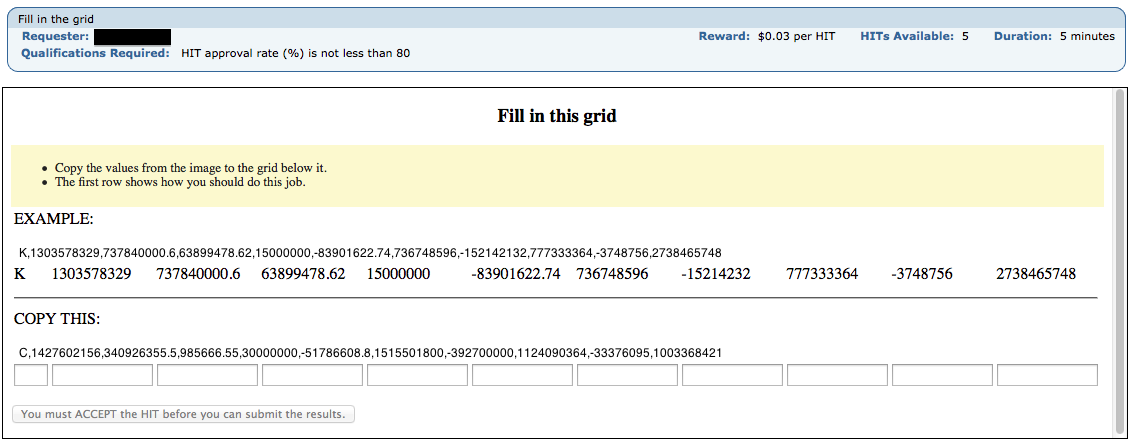
\includegraphics[width=6.5in]{images/mturk_fuzz_task}
  \caption{The page presented to Mechanical Turk workers to perform data entry tasks in order to collect actual human data entry errors (see Section~\ref{sec:user_study}).\label{fig:mturk_task}}
\end{figure*}



Our ground truth data was drawn from \texttt{3q2000.xls}, a
spreadsheet from the EUSES repository that contains selected financial
information from Fannie Mae. We saved the data as a comma-separated
value file (.csv). Mechanical Turk workers were then paid 3 cents to
enter 10 of these values at a time into a web form designed to look
like a spreadsheet, shown in Figure~\ref{fig:mturk_task}. To prevent
copying and pasting, we generate an image containing the
comma-separated values.  Each worker had the opportunity to perform up
to seven data entry tasks.

In all, we collected 200 responses from 46 distinct users. Out of
these responses, 14 had omitted data and 50 contained errors, for an
overall error rate of 35\%.

We then inserted this erroneous data back into the spreadsheet and
ran \checkcell{} to see whether it found any of these errors. Recall
that \checkcell{} cannot find any errors that do not have an unusual
impact on any of the calculations.
